%!TEX root = ../thesis.tex


\if pdf
    \graphicspath{{Chapter4/Figs/Raster/}{Chapter4/Figs/PDF/}{Chapter4/Figs/}}
\else
    \graphicspath{{Chapter4/Figs/Vector/}{Chapter4/Figs/}}
\fi

\chapter{Hidden Markov Models}

Until now, we have considered visible states in a sense that the sequence of states was known, we refer to these models as \textit{visible Markov Models}.
In this section we will consider a situation in which we do not observe the states directly but only as a "guess" given other visible observations that are available. 
These "visible" observations are labeled as emissions emitted by the respective hidden state. Thus, the observations are assumed to be generated by certain hidden stochastic process, i.e. a Markov Chain.\footnote{Models that
comprise unobserved random variables, e.g. Hidden Markov Models, are called \textbf{latent variable models}, \textbf{missing data models}, or also \textbf{models with incomplete data}}
In general, we could assume that the state and emission space is not necessarily finite, but we will follow the classical definition by \citep{Rabiner1989} and \citep{Elliott1995} of Hidden Markov Model (hereinafter "HMM") and assume that at least state space is finite.

\section{Discrete Hidden Markov Model}

A Discrete Hidden Markov Model is one where the observations are assumed to be a sequence of discrete symbols or categorical variables. It defines a family of models that are
commonly used in statistical signal processing, speech recognition, computational biology, and other fields. \citep{Rabiner1989}

There are two main models under the umbrella of Discrete Hidden Markov Models, namely \textit{Categorical Hidden Markov Model} and \textit{Multinomial Hidden Markov Model}. The difference between them 
is in the way we are interpreting the emissions. In case of Categorical HMM, we assume that the emissions are categorical variables, i.e. they are represented by a single integer value,
meaning that each emission belongs to one of the $M$ possible categories. On the other hand, in case of Multinomial HMM, we assume that the emissions at each time step are a result of a multinomial experiment,
i.e. certain number of trials with $M$ possible outcomes. In other words, each emission is represented by a vector of length $M$ with only one element equal to 1 and the rest 0 since the number of trials is fixed to 1.
Such vector definition would change if we had more than one trial in single time step, but we will not consider such case in this work since it is not applicable to the problem at hand. We always assume that the number of trials is fixed to 1
and thus each observation might be represented by a vector of length $M$ with only one element equal to 1 and the rest 0 or by a single integer value for the purpose of Categorical HMM. This vector representation is also called \textit{1-of-M encoding}, but 
we will use the representation of integer values since it is easier to interpret and more efficient in our case.

Revisiting previous section, we have defined a transition matrix $\textbf{A}$ and initial distribution $\textbf{p}$ for a homogeneous Markov Chain. Both of these parameters are used to describe the hidden stochastic process.
In order to describe the emissions, we will define an $N \times M$ \textit{emission matrix}\footnote{Also referred to as \textbf{observation matrix} and \textbf{observations} respectively} $\textbf{B}$ as follows:

\begin{equation}
    \textbf{B} = \begin{pmatrix}
    b_1(y_1) & b_1(y_2) & \ldots & b_1(y_M) \\
    b_2(y_1) & b_2(y_2) & \ldots & b_2(y_M) \\
    \vdots & \vdots & \ddots & \vdots \\
    b_N(y_1) & b_N(y_2) & \ldots & b_N(y_M) \\
    \end{pmatrix}
\end{equation}

\noindent where $N$ represents number of states and $M$ number of possible emission symbols.

Probabilistically each element of the matrix represents conditional probability of emitting symbol $k$ for all $k = 1,2,\ldots,M$, given state $i$: 

\begin{equation}
    b_{i}(k) = \mathbb{P}(Y_t = k|X_t = i) 
\end{equation}

As stated at the beginning of this section, observer does not have access to the hidden states, but only to the emissions emitted by the hidden states. 
Thus, observing only another stochastic process $\{Y_t, t \in \mathbb{N}_0\}$ linked to hidden Markov Chain s.t. it governs the distribution of $Y_t$. 
In other words, entire statistical inference, even in terms of the hidden Markov process, is based on the observed sequence of emissions $\{Y_t\}$.

Considering the discrete time index $t$, Hidden Markov model is bivariate discrete-time stochastic process $\{X_t,Y_t\}$, where $\{Y_t\}$ is a sequence of conditionally 
independent and identically distributed random variables with a probability distribution determined by the hidden state $i$ at time $t$. \citep{Rabiner1989}

Note that there are three common types of Hidden Markov Models depending on structure of the underlying hidden Markov Chain according to \citep{Nelwamondo2006}. These are namely (a) left-to-right, 
(b) two-parallel left-to-right and (c) ergodic. First model bears a property that the next state index is always greater than or equal to the current state index s.t. the final state is absorbing.
Two-parallel left-to-right model allows for two parallel paths taken by the Markov Chain and lastly in ergodic model, all states are connected.
For the purpose of this work we will only consider models with ergodic property as shown in Figure \ref{fig:ergodic}.

Above we specified an emission matrix $\textbf{B}$ as a discrete probability distribution of the emissions, given the hidden state, that take on values from a finite set of $M$ possible emissions. $\{Y_t\}$ is then a sequence of conditionally 
independent and identically distributed discrete random variables that follow a categorical distribution with $M$ possible outcomes, i.e. each emission symbol $k$ is given a probability of being emitted by the hidden state $i$
 as stated by \citep{Paisley2009}:

\begin{gather}
    Y | X = i \sim \text{Cat}(M;b_i(y_1),\ldots,b_i(y_M)), \quad \forall i \in I \\
    f(y|x=i) = \prod\limits_{k=1}^M b_i(k)^{\mathbbm{1}{\{y=k\}}}
\end{gather}
 
Important property of the categorical distribution in Bayesian statistics is that it is a generalization of the Bernoulli distribution for $M > 2$ 
outcomes and also a conjugate prior for the Dirichlet distribution. In some instances, as expressed by \citep{Paisley2009}, we also use Dirichlet distribution with parameters $\alpha_1=\ldots=\alpha_M$ 
as it is a special case called uniform prior for the categorical distribution. The same approach is also applicable other parameters of the model, i.e. 
transition matrix $\textbf{A}$ and initial distribution $\textbf{p}$.

Usually, as mentioned in \citep{Agresti2007}, we generalize the categorical distribution to a multinomial distribution in which case the number of samples is fixed to 1. 
In other words, the emission space is not 1-to-M encoded but rather 1-of-M encoded s.t. the probability mass function is:

\begin{gather}
    Y | X = i \sim \text{Multinomial}(1;M;b_i(y_1),\ldots,b_i(y_M)), \quad \forall i \in I \\
    f(\textbf{y},n=1|x=i) = \prod_{k=1}^M b_i(k)^{y_{k}}, \quad \sum_{k=1}^M y_{k} = 1
\end{gather}

\noindent where $\textbf{y}$ is a vector of length $M$ with only one element equal to 1 and the rest 0. 

HMM with finite state and emission space as described above is also called \textit{discrete Hidden Markov Model}. Same definition is also applicable for continuous emission space, where the probability density function is 
often a Gaussian distribution with mean vector $\mathbf{\mu}$ and covariance matrix $\Sigma$ or Poisson distribution with parameter vector $\boldsymbol{\lambda}$.

An important note, as per \citep{Bishop2006} and \citep{Ramaprasad2004}, is that the emissions are not necessarily independent, but only conditionally independent given the hidden state, which implies that the process $\{Y_t\}$ is not a Markov Chain, as opposed to process $\{X_t\}$,
but we may view it as an extension of Mixture Models with certain dependencies between the emissions. For example, in a case where we have a Markov Chain with finite $N$ hidden states and emissions modelled by Gaussian distributions, 
we refer to such model as \textit{Gaussian Hidden Markov Model}\footnote{In some literature as \citep{Capp2005} also \textbf{normal Hidden Markov Model}} s.t. marginal distribution of $Y_t$ is a mixture of Gaussian distributions.

Since HMM is categorized as a sequence model, we are generally interested in a joint probability distribution of the hidden states and the emissions when examining 
time series data or any other sequential data. Such joint probability distribution given parameters vector $\theta = (\textbf{A},\textbf{B},\textbf{p})$ is, as described by \citep{Rabiner1989}, 
expressed by the following equation:

\begin{align}
    \mathbb{P}(\textbf{X}, \textbf{Y}| \theta) = & \mathbb{P}(X_0 = x_0) \mathbb{P}(Y_0 = y_0|X_0 = x_0) \notag \\ 
                                                 & \prod_{t=1}^T \mathbb{P}(X_t = x_t|X_{t-1} = x_{t-1}) \mathbb{P}(Y_t = y_t|X_t = x_t) \\
                                               = & p_{x_0} b_{x_0}(y_0) \prod_{t=1}^T a_{x_t,x_{t-1}} b_{x_t}(y_t)
\end{align}

\noindent where $\textbf{X} = \{x_0,x_1,\ldots,x_T\}$ and $\textbf{Y} = \{y_0,y_1,\ldots,y_T\}$ are the sequences of hidden states and emissions respectively. 

One possibility of graphically representing such joint probability distribution is by using a graphical 
model as shown in Figure \ref{fig:HMM}. 

\begin{figure}[htbp]
\begin{center}
    \begin{tikzpicture}[->,>=stealth',shorten >=1pt,auto,node distance=2.5cm,semithick]
    \node[state, minimum size=1.2cm]         (A)                    {$x_{t-1}$};
    \node[state, minimum size=1.2cm]         (B) [right of=A]       {$x_{t}$};
    \node[state, minimum size=1.2cm]         (C) [right of=B]       {$x_{t+1}$};

    \node[left of=A]  (prev) {$\dots$};
    \node[right of=C] (next) {$\dots$};

    \path (prev) edge node [above] {} (A)
    (A)    edge node [above] {} (B)
    (B)    edge node [above] {} (C)
    (C)    edge node [above] {} (next);

    \node [draw,circle,below of=A, node distance=2cm, minimum size=1.2cm] (WA) {$y_{t-1}$};
    \node [draw,circle,below of=B, node distance=2cm, minimum size=1.2cm] (WB) {$y_{t}$};
    \node [draw,circle,below of=C, node distance=2cm, minimum size=1.2cm] (WC) {$y_{t+1}$};

    \path (A) edge [->] (WA)
    (B) edge [->] (WB)
    (C) edge [->] (WC);
    \end{tikzpicture}
\end{center}
\caption[Left-to-right state and emission dependence in Hidden Markov Model]{An HMM with 4 hidden states and 2 discrete emissions denoted by $x_1$ and $x_2$.}
\label{fig:HMM}
\end{figure}

We may also visualize conditional relationship with a graphical model in Figure \ref{fig:ergodic} representing a structure of HMM with 3 hidden states $\{S_1,S_2,S_3\}$ and 2 emission symbols $\{E_1,E_2\}$ where the nodes represent the relationship 
imposed by the transition matrix $\textbf{A}$ and emission matrix $\textbf{B}$:

\begin{figure}[htbp]
    \begin{center}
    \begin{tikzpicture}[]
    % states
    \node[state, minimum size=1.2cm] (s1) at (0,2) {$S_1$}
        edge [loop above]  node[auto,above] {$a_{11}$}();
    \node[state, minimum size=1.2cm] (s2) at (3,2) {$S_2$}
        edge [<-,bend right=45] node[auto,swap] {$a_{12}$} (s1)
        edge [->,bend left=45] node[auto,above] {$a_{21}$} (s1)
        edge [loop above] node[auto,above] {$a_{22}$} ();
    \node[state, minimum size=1.2cm] (s3) at (6,2) {$S_3$}
        edge [<-,bend right=70] node[auto,swap] {$a_{13}$} (s1)
        edge [->,bend left=60] node[auto,above] {$a_{31}$}(s1)
        edge [<-,bend right=45] node[auto,swap] {$a_{23}$} (s2)
        edge [->,bend left=45] node[auto,above] {$a_{32}$} (s2)
        edge [loop above] node[auto,above] {$a_{33}$} ();
    % observations
    \node[observation, minimum size=1cm] (y1) at (1.5,-1.5) {$E_1$}
        edge [lightedge] node[auto,below,xshift=-20pt] {$b_{S_1}(E_1)$} (s1)
        edge [lightedge] (s2)
        edge [lightedge] (s3);
    \node[observation, minimum size=1cm] (y2) at (4.5,-1.5) {$E_2$}
        edge [lightedge] (s1)
        edge [lightedge] (s2)
        edge [lightedge] node[auto,swap] {$b_{S_3}(E_2)$} (s3);
    \end{tikzpicture}
    \end{center}
    \caption[Graph interpretation of Discrete Hidden Markov Model]{An HMM with 3 hidden states and 2 emission symbols denoted by $E_1$ and $E_2$.}
    \label{fig:ergodic}
\end{figure}
    
There are 3 main assumptions of Hidden Markov Models as a consequence of the properties of Markov processes,
as suggested by \citep{Oliver2013} and \citep{Capp2005}:

\begin{itemize}
    \item[1)] \textbf{Markov memoryless assumption} - this assumption states that the next hidden state $X_{t+1}$ depends only on the current state $X_t$, so that the transition probabilities are defined as:

        \begin{equation}
            \mathbb{P}(X_{t+1} = j| X_{t} = i,X_{t-1} = i_{t-1}, \ldots,X_{0} = i_0) = \mathbb{P}(X_{t+1} = j| X_{t} = i) \quad \forall i,j \in I
        \end{equation}

        It is also possible to assume that the states in HMM are dependent beyond the current state therefore giving rise to \textit{k-order HMM} 
        where the conditional distribution of the next state depends on the current state and the previous $k$ states $X_{t-k}, X_{t-k+1}, \ldots, X_{t-1}$. \citep{Capp2005}

    \item[2)] \textbf{Stationary assumption} - The transition matrix $\textbf{A}$ is time invariant s.t. transition probabilities only depend on the time interval between the transitions, 
    thus for all $t \neq s$:

        \begin{equation}
            \mathbb{P}(X_{t+1} = j| X_{t}= i) = \mathbb{P}(X_{s+1} = j| X_s = i) \quad \forall i,j \in I
        \end{equation}

        However, when we abstract from this assumption, we may consider a \textit{non-stationary HMM} where the transition matrix is time-dependent, i.e. depends on time index $t$.

    \item[3)] \textbf{Emission independence assumption} - Emissions are independent, s.t. if we have an emission sequence $\textbf{Y} = \{y_1,y_2,\ldots,y_T\}$ then:

        \begin{equation}
            \mathbb{P}(\textbf{Y}|X_1 = x_1,\ldots,X_T = x_T) = \prod_{t=1}^T \mathbb{P}(Y_t = y_t|X_t = x_t)
        \end{equation}

        When there is a dependence between the emissions in a way that the emission at time $t$ depends on the previous emissions, conditionally on the hidden state sequence $\{X_k\}$, $\{Y_k\}$
        forms a (non-homogeneous) Markov Chain, therefore jointly representing a generalization of HMM called \textit{Markov-switching Models}\footnote{Also, \textbf{Markov jump system}.}. \citep{Capp2005}

\end{itemize}

There are mainly 3 fundamental problems in HMM that need to be resolved as depicted by \citep{Oliver2013} and \citep{Ching2005}:
\begin{itemize}
\item[1.] \textbf{Evaluation problem} - Given a model denoted as $\theta = (\textbf{A},\textbf{B},\textbf{p})$ and an emission sequence 
                                        $\textbf{Y} = y_1, y_2,\ldots,y_T$, how to efficiently compute the probability that the model generated the observation 
                                        sequence, in other words, what is $\mathbb{P}(\textbf{Y}|\theta)$? 
\item[2.] \textbf{Decoding problem} - What is the most likely sequence of hidden states that could have generated the emission sequence \textbf{Y}? 
                                      Thus, we would like to find $\textbf{X} = \underset{\textbf{X}}{\arg\max} \mathbb{P}(\textbf{Y},\textbf{X}|\theta)$, 
                                      where $\textbf{X}$ is the hidden state sequence. 
\item[3.] \textbf{Learning problem} - Given a set of emission sequences find $\theta$ that best explains the emission sequence $\textbf{Y}$. 
                                      Thus, find the vector of parameters $\theta$ that maximizes $\mathbb{P}(\textbf{Y}|\theta)$. 
\end{itemize}

The most traditional approaches in solving these 3 fundamental problems differ and one may not suffice in solving all three. 
The evaluation problem is usually solved by \textbf{Forward-Backward algorithm}\footnote{Focusing on the most widely used implementation called \textbf{alpha-beta algorithm}.}, the decoding problem by well-known \textbf{Viterbi algorithm} 
and the last learning problem by \textbf{Baum-Welsch algorithm} which is a special case of Expectation-maximization (EM) algorithm.
 All three algorithms are described in the following chapter.
 
\section{Continuous HMM}
 
If we were to consider a continuous emission space, we could plot the joint probability distribution of the hidden states and the emissions to see that 
the marginal distribution of the emissions is not that easily tractable and may not necessarily be unimodal. For example, in \textit{Gaussian Hidden Markov Model} (GHMM) setting, 
marginal distribution of the emissions is a mixture of Gaussian distributions that are either univariate or multivariate depending on the feature space. \citep{Bishop2006}

Although, most of the time we consider unimodal distributions for our data it might not be the case for incomplete data, i.e. data with missing values.
For example, statistical inferences about the subpopulations within the overall population require such tools in cases where the subpopulations significantly differ 
and may be interpreted the same way as hidden variables in case of Hidden Markov Models. With the extension of Mixture Models we could possibly consider any
distribution as a component of the mixture, but since Gaussian distributions are able to approximate any density arbitrarily well, we will focus on them in the following section.

\subsection{Mixture Distributions}

Let $\textbf{Y}$ denote a p-dimensional random vector with probability density function $f_{\textbf{Y}}(y_1,\ldots,y_p)$ on $\mathbb{R}^p$. 
This probability density function is defined as a convex combination of $M$ component probability densities as follows from \citep{McLachlan2000}: 

\begin{equation} \label{eq:mixture}
    f_{\textbf{Y}}(y_1,\ldots,y_p) = \sum_{i=1}^{M} \pi_i f_i(y_1,\ldots,y_p)
\end{equation}

where $f_i$ is a component density of the mixture and $\pi_i$ a mixing proportion or mixture weight with following properties:

\begin{equation}
    0 \leq \pi_i \leq 1 \quad \forall i \in \{1,2,\ldots,M\}
\end{equation}

and

\begin{equation}
    \sum_{i=1}^{M} \pi_i = 1
\end{equation}

Therefore, the probability density $f_{\textbf{Y}}$ given by Equation \ref{eq:mixture} is referred to as a g-component finite mixture density, conversely $F_{\textbf{Y}}$ 
as a g-component finite mixture distribution. 

Equation \ref{eq:mixture} also assumes that the number of components $M$ is fixed but in many applications this is not the case, and we have to infer 
the number of components which are required to adequately describe the data. One way we can avoid this problem is by assuming that the number of components is 
sufficiently large or infinite, and then use a model selection criterion to select the number of components that best fits the data as suggested by \citep{Sammut2011} and \citep{Rasmussen1999}.
Furthermore, mixing proportions $\pi_i$ are also unknown and have to be estimated along with the respective parameters of the component densities.

Analogously to previous definition we can define a finite mixture of random vector $\textbf{Y}$ as \citep{Bishop2006}:

\begin{equation}
    f(y,x) = g(x) f(y|x)
\end{equation}

where $X$ is defined as a random variable following a multinomial distribution with a vector of parameters $\pi = \{\pi_1,\ldots,\pi_M\}$ and $g(x)$ as its 
probability density function. Summing over all possible values of $X$ we obtain the marginal density of random vector $\textbf{Y}$:

\begin{equation}
    f_{\textbf{Y}}(y_1,\ldots,y_p)= \sum_{i=1}^{M} \mathbb{P}(X=i) f_{\textbf{Y}}(y_1,\ldots,y_p|X=i)
\end{equation}
    
where $\mathbb{P}(X=i) = \pi_i$ and $f_{\textbf{Y}}(y_1,\ldots,y_p|X=i) = f_i(y_1,\ldots,y_p)$ are the mixing proportions and component densities respectively thus arriving at the same definition 
as in Equation \ref{eq:mixture}.

\subsection{Gaussian Mixture Models}

The Gaussian mixture model (GMM) is a probabilistic model that assumes all the data points are generated 
from a mixture of a finite number of Gaussian distributions. The component distributions are often chosen to be members of the same parametric family,
such as Gaussian distributions with respective mean and covariance parameter. Assuming that the number of components is $K$
the probability density function of the Gaussian mixture model can be expressed as follows \citep{Bishop2006}:

\begin{equation}
    f(y|\mu,\Sigma) = \sum_{k=1}^{K} \pi_k \mathcal{N}(y|\mu_k, \Sigma_k)
\end{equation}

where $\mu_k$ and $\Sigma_k$ are the mean and covariance matrix (symmetric and positive semi-definite) of the $k$-th Gaussian component. 

Thus, the vector of parameters is $\theta = \{k \in \mathbb{N}: (\pi_k,\mu_k,\Sigma_k)\}$. Probability density function of each component of GMM depends on the dimensionality of the data.
Let the dimensionality of the data be $d>1$ then the random vector $\textbf{Y}=(y_1,\ldots,y_d)$ has the probability density function of the $k$-th component 
defined as following multivariate Gaussian distribution:

\begin{equation}
    f_k(\textbf{Y}) = \frac{1}{{(2\pi)}^{d/2}|\Sigma_k|^{1/2}} \exp\left(-\frac{1}{2}{(\textbf{Y}-\mu_k)}^T\Sigma_k^{-1}(\textbf{Y}-\mu_k)\right)
\end{equation}

where $|\Sigma_k|$ denotes the determinant of d x d covariance matrix $\Sigma_k$ and $\mu_k$ is a d-dimensional mean vector. Therefore, the conditional distribution of $Y$ given component $k$ is:

\begin{equation}
    \textbf{Y}|k \sim \mathcal{N}_d(\mu_k,\Sigma_k)
\end{equation}

If we consider $d=1$ we say that the random variable $Y$ has a univariate Gaussian distribution with mean $\mu_k$ and variance $\sigma_k^2$ and there the 
mixture model is called a \textit{univariate normal (Gaussian) mixture model} as in Fig \ref{fig:1_d_guaussian_mix} with number of components $M=3$. In case of $d>1$ we refer to the model as \textit{multivariate normal (Gaussian) mixture model}, e.q. in Fig \ref{fig:2_d_guaussian_mix} 
where $d=2$ and $M=3$.

\begin{figure}[htbp]
    \centering
    \begin{subfigure}[b]{0.48\textwidth}
        \centering
        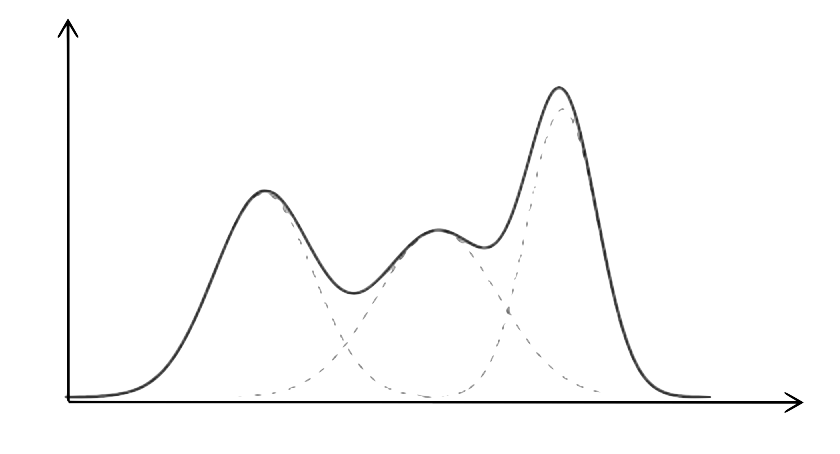
\includegraphics[width=\textwidth]{Figs/d_1_gaussian_mix.png}
        \caption{d = 1}
        \label{fig:1_d_guaussian_mix}
    \end{subfigure}
    \hfill
    \begin{subfigure}[b]{0.48\textwidth}
        \centering
        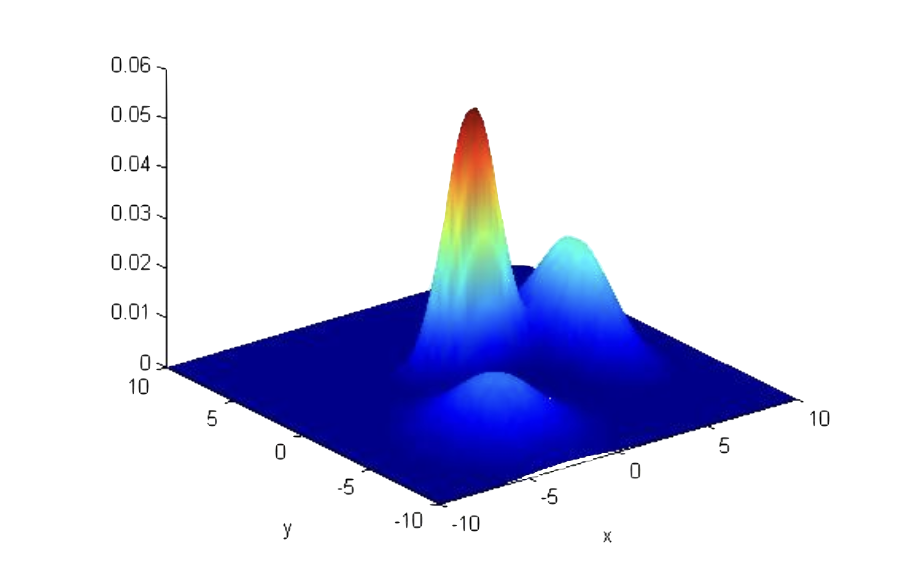
\includegraphics[width=\textwidth]{Figs/d_2_gaussian_mix.png}
        \caption{d = 2}
        \label{fig:2_d_guaussian_mix}
    \end{subfigure}
        \caption*{\textbf{Source:} \href{https://web.iitd.ac.in/~sumeet/GMM_said_crv10_tutorial.pdf}{\textit{A short tutorial on Gaussian Mixture Models by Mohand Saïd Allili}}}
        \caption[Probability distribution of Gaussian Mixture Model]{Probability distribution of Gaussian Mixture Model with $M=3$ components for $d=1$ and $d=2$ respectively.}
    \label{fig:gaussian_mix}
\end{figure}

The motivation for using the Gaussian mixture model is that it is a universal approximation of densities, i.e. it can approximate any density arbitrarily well as stated by \citep{Bishop2006}.
In a setting of possible stock price prediction we may consider looking at asset returns as a mixture of Gaussian distributions, where each component represents a different regime of the market.
This was first considered by \citep{Fama1965} in estimating densities of asset returns and later further developed by other authors. Indeed, the financial markets were shown to be
characterized by different regimes that manifest themselves in the implication on the mean and variance of the returns. \citep{Hamilton1989}

We aim to briefly explain only one regime that deviates from the "usual" view of the asset returns distribution, which was first 
introduced by \citep{Black1976} and later by \citep{Christie1982}. This regime or effect is called \textit{leverage effect}, 
and it is defined as a negative correlation between the returns and the volatility of the asset. Such effect is often observed in
the financial markets and is usually attributed to the fact that the expected asset returns tend to increase during 
pronounced market downturns, as well as during periods of higher volatility. \citep{Aydemir2007}

Such behavior might be captured by a 2-component mixture of Gaussian distributions, where the first component represents the "usual" regime 
of the market and the second component represents the "leverage" regime. The former component often exhibits near zero mean, while the latter 
is accompanied by negative mean and much higher variance and correlations to address the existence of the asymmetry and leptokurtosis in the distribution of 
asset returns. \citep{Paolella2015}

This is providing us with a motivation to consider a Gaussian mixture model as a generative model for the asset returns and volatility which 
we will further use in the context of Hidden Markov Models in prediction of the market states.

As for the estimation of the parameters of the Gaussian mixture model, we will use the Expectation-maximization (EM) algorithm which is a general
approach to maximum likelihood estimation in the presence of missing or hidden data. The details of the algorithm are described in the following chapter
focused on the parameter estimation. \citep{Dempster1977}

\subsection{Gaussian HMM}

As we have shown in the previous section, Hidden Markov Models are a generalization of Mixture Models with dependencies between the hidden states.
In section dedicated to \textit{Discrete HMM} we have shown that the marginal distribution of the emissions given state is categorical distribution. 
Since a suitable choice for the emission distribution is a Gaussian distribution, we may distinguish between two types of Gaussian Hidden Markov Models,
namely \textit{Gaussian-Mixture HMM} and \textit{Gaussian HMM}. The former is a generalization of the latter, where the marginal distribution of the emissions is a mixture of Gaussian distributions. \citep{Bishop2006}

In case of Gaussian HMM, the marginal distribution of the emissions is a $d$-dimensional Gaussian distribution with $N \times d$ mean vector $\mu$ and vector $\Sigma$ of length $N$ of $d \times d$ covariance matrices, thus the number of components $M=1$. 
Depending on the dimensionality of the data, we may consider univariate or multivariate Gaussian distribution. The probability density function of the $d$-dimensional Gaussian distribution 
for each hidden state $i$ is defined as follows:

\begin{equation}
    b_i(y_t) = \frac{1}{{(2\pi)}^{d/2}|\Sigma_i|^{1/2}} \exp\left(-\frac{1}{2}{(y_t-\mu_i)}^T\Sigma^{-1}_i(y_t-\mu_i)\right)
\end{equation}

where $y_t$ is a $d$-dimensional vector of emissions at time $t$. Parameters of such HMM model are therefore $\theta = \{\textbf{A},\textbf{p},\mu,\Sigma\}$.

Taking into account $M>1$ components, we arrive at the Gaussian-mixture HMM, where the marginal distribution of the emissions is a mixture of Gaussian distributions. 
The probability density function of the $d$-dimensional Gaussian mixture distribution for each hidden state $i$ is defined as follows:

\begin{equation}
    b_i(y_t) = \sum_{k=1}^{M} \frac{\pi_{i,m}}{{(2\pi)}^{d/2}|\Sigma_{i,k}|^{1/2}} \exp\left(-\frac{1}{2}{(y_t-\mu_{i,k})}^T\Sigma^{-1}_{i,k}(y_t-\mu_{i,k})\right)
\end{equation}

where $\pi_{i,k}$ is the mixing proportion of the $k$-th component of the mixture and $\mu_{i,k} \in \mathbb{R}^d$ and $\Sigma_{i,k} \in \mathbb{R}^{d \times d}$ are the mean and covariance matrix of the $k$-th component respectively. Suddenly the number of parameters
increases linearly with the number of components $M$ and thus the model becomes more complex. Parameters of such HMM model are therefore $\theta = \{\textbf{A},\textbf{p},\pi,\mu_{i,k},\Sigma_{i,k}\}$ for $i=1,\ldots, N$ and $k=1,\ldots, M$.

One convenient way to represent this model, according to \citep{Yu2015}, is to view it as a generative model producing a sequence of emissions $\textbf{Y} = \{y_1,\ldots,y_T\}$ as follows:

\begin{equation}
    y_t = \mu_{i} + r_t(\Sigma_{i})
\end{equation}

where the state $i$ is determined by the transitions in the Markov Chain and $r_t$ is a random $d$-dimensional vector drawn from the Gaussian distribution with zero mean and covariance matrix $\Sigma_{i}$.
Below you can see a graphical representation of such models:

\begin{figure}[htbp]
    \begin{center}
        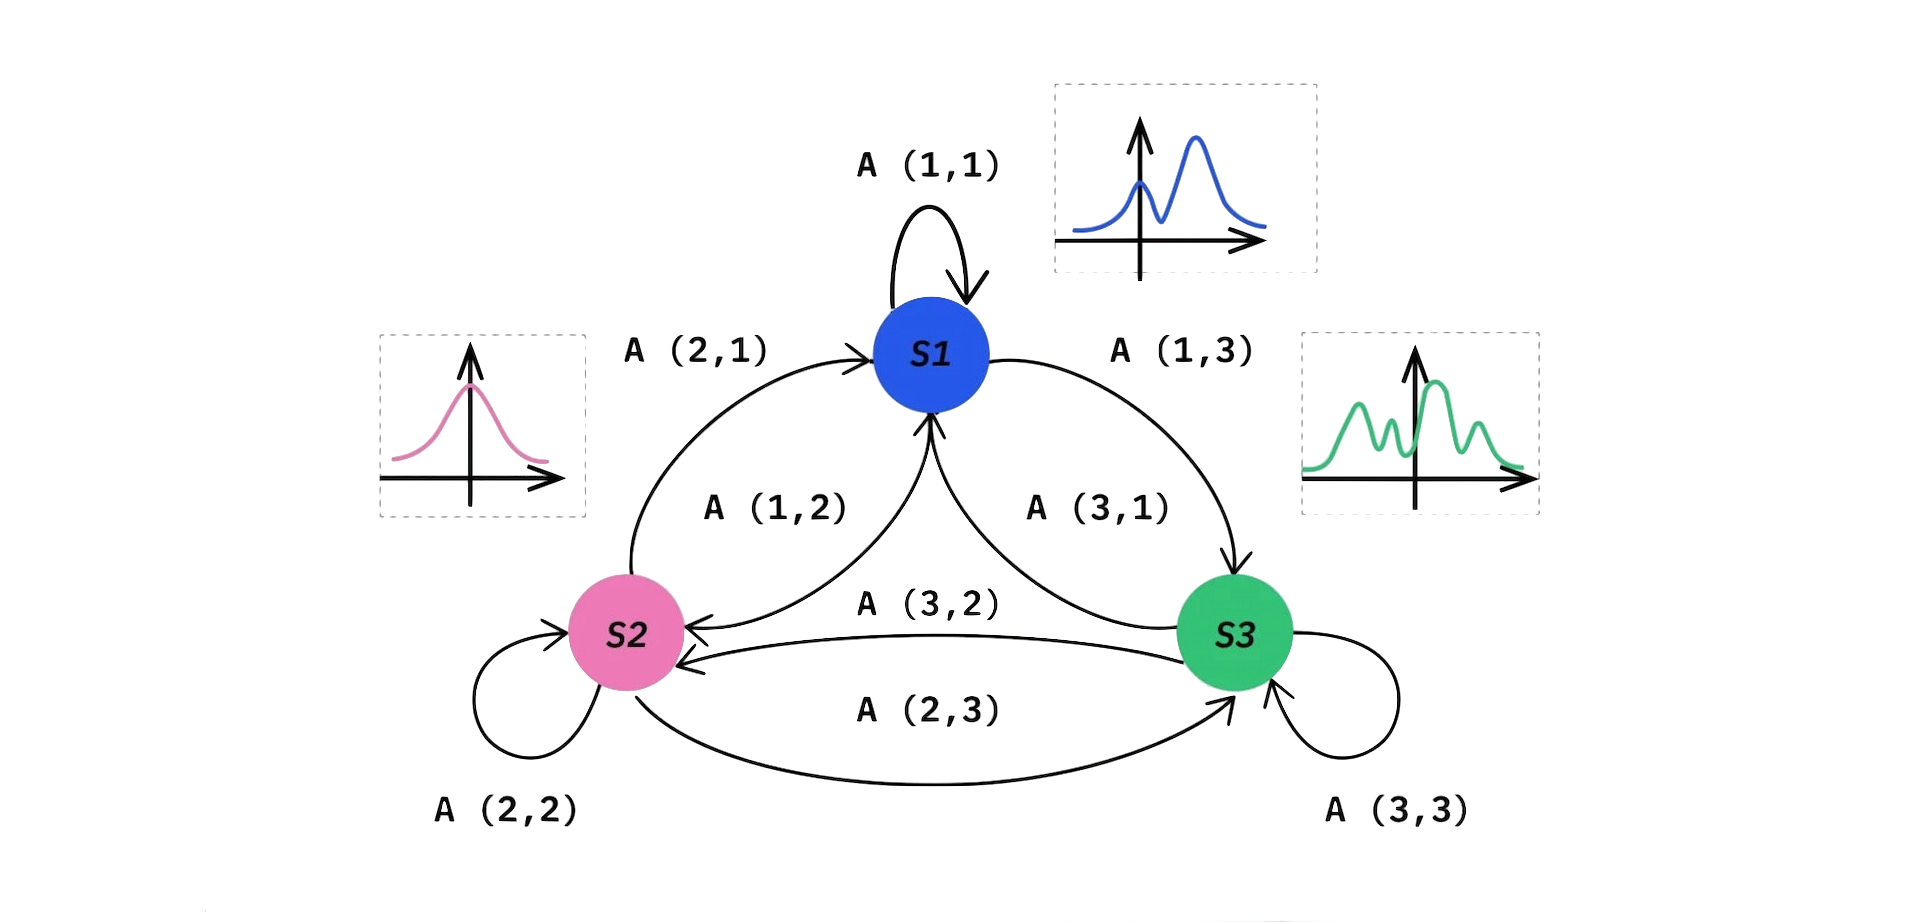
\includegraphics[width=1.0\textwidth]{Figs/gaussian_hmm.png}
        \caption*{\textbf{Source:} \href{https://tooploox.com/improving-hidden-markov-models-tooploox-at-neurips-2022s}{\textit{Improving Hidden Markov Models – Tooploox at NeurIPS 2022}}}
        \caption[Diagram of Gaussian Hidden Markov Model representation]{Graphical representation of Gaussian-Mixture HMM. Each hidden state S1, S2 and S3 is associated with a Gaussian mixture distribution with $M$ components. A(i, j) denotes the transition probability from state i to state j.}
        \label{fig:guaussian_hmm}
    \end{center}
\end{figure}

\section{Hidden Semi-Markov Model}

One of the limitations mentioned in the chapter dedicated to Markov Renewal Processes is the fact that the time spent in a state is geometrically distributed which is not
always the case in real-world applications. In order to address this issue, we may consider a generalization of the Hidden Markov Model called \textit{Hidden Semi-Markov Model} (HSMM) where
the time spent in a state follows a general distribution, e.g. Poisson, Negative binomial. \citep{Yu2015}

In classical HMM setting, each observation at time $t$ is generated by the hidden state $X_t$. After emitting the observation, the model transitions to a new state $X_{t+1}$ according to 
the transition probabilities. In case of HSMM, the model stays in the same state $i$ for a random number of time steps before transitioning to state $j$, which is called waiting time and is denoted by $W_{i,j}t$.
This means that the original observation sequence $\textbf{Y} = \{y_1,\ldots,y_T\}$ now consists of multiple subsequences $\textbf{C}_1,\ldots,\textbf{C}_L$ where each element in subsequence $\textbf{C}_l$ is generated by the same hidden state. \citep{Dasu2011}
The number of subsequences $L$ as well as the length of each subsequence $C_l$ is governed by the waiting time distribution, which is why this model is sometimes referred to as \textit{Explicit-duration HMM}. \citep{Yu2015} 

This is an important distinction from the classical model assumption of the HMM where each state can only generate one observation per time step. Thus, the number of observations produced by the state $i$ is determined by the time spent in such state, i.e. duration $d$. 
This relationship is depicted in Figure \ref{fig:HSMM} where we clearly see that e.g. the number of observations generated by the state $x_{l-1}$ is equal to the duration $d=3$. 


\begin{figure}[htbp]
    \begin{center}
        \begin{tikzpicture}[->,>=stealth',shorten >=1pt,auto,node distance=3.5cm,semithick]
        \node[state, minimum size=1.2cm]         (A)                    {$x_{l-1}$};
        \node[state, minimum size=1.2cm]         (B) [right of=A]       {$x_{l}$};
        \node[state, minimum size=1.2cm]         (C) [right of=B]       {$x_{l+1}$};
    
        \node[left of=A]  (prev) {$\dots$};
        \node[right of=C] (next) {$\dots$};
    
        \path (prev) edge node [above] {} (A)
        (A)    edge node [above] {} (B)
        (B)    edge node [above] {} (C)
        (C)    edge node [above] {} (next);
    
        \node [draw,circle,below of=A, node distance=2cm, minimum size=1.2cm] (WA) {$y_{t-2}$};
        \node [draw,circle,right of=WA, node distance=1.25cm, minimum size=1.2cm] (WA2) {$y_{t-1}$};
        \node [draw,circle,left of=WA, node distance=1.25cm, minimum size=1.2cm] (WA3) {$y_{t-3}$};
        
        \node [draw,circle,below of=B, node distance=2cm, minimum size=1.2cm] (WB) {$y_{t}$};
        
        \node [draw,circle,below of=C, node distance=2cm,minimum size=1.2cm, xshift=-1cm] (WC) {$y_{t+1}$};
        \node [draw,circle,right=1cm of WC, minimum size=1.2cm] (WC2) {$y_{t+2}$};
    
        \path 
        (A) edge [->] (WA2)
        (A) edge [->] (WA)
        (A) edge [->] (WA3)
        (B) edge [->] (WB)
        (C) edge [->] (WC)
        (C) edge [->] (WC2);

        \end{tikzpicture}
    \end{center}
    \caption[Left-to-right state and emission dependence in Hidden Markov Model]{HSMM with left-to-right state and emission dependence. The number of observations generated by the state $x_l$ is equal to the duration $d$. State $x_{l-1} \neq x_l$ and also $x_l \neq x_{l+1}$.}
    \label{fig:HSMM}
\end{figure}

It is obvious that the only difference between the classical discrete HMM and HSMM is the way the observations are generated. In case of HSMM, the observations are generated by the same state for a random number of time steps and therefore
the transition probabilities given by matrix $\textbf{A}$ ought to be adjusted accordingly, but emission probabilities remain the same, i.e. the conditional (discrete or continuous) distribution of emissions given state is defined identically. In order to account for the duration of the chain in each state, we will introduce,
as suggested by e.g. \citep{Bulla2013}, probability distribution called \textit{sojourn time distribution} $d_{j}(u)$ which is defined as follows:

\begin{equation}
    d_{i}(u) = \mathbb{P}(X_{t+u+1} \neq i,X_{t+u} = i,\ldots,X_{t+2} = i|X_{t+1} = i, X_t \neq i)
\end{equation}

where the sojourn time distribution $d_{i}(u)$ is the probability of staying in state $i$ for $u$ time steps and then transitioning to another state. There is a possibility of using discrete or continuous valued random variable for duration
but in case of HSMM we assume that the sojourn time distribution $d_i(u)$ is discrete valued, i.e. $u = \{1,2,3,\ldots,D\}$ where $D$ is the maximum possible duration in respective state, as stated in \citep{Yu2010}. The most popular choices 
of the sojourn time distribution are Poisson, negative binomial or geometric distribution
depending on the application. As for the transition probabilities, we are interested in the probability of transitioning from state $i$ to state $j$ but only if $i \neq j$ since the probability of 
staying in the same state is not governed by the geometric distribution anymore. \citep{Abdullah2022} Hence, the transition probabilities are defined as follows:

\begin{equation}
    a_{i,j} = \mathbb{P}(X_{t+1} = j|X_{t+1} \neq i, X_t = i)
\end{equation}

where $p_{i,i} = 0$, thus the transition matrix $\textbf{A}$ has its diagonal elements equal to zero and is valid stochastic or Markov matrix since $\sum_{i \neq j} a_{i,j}= 1$.

\section{Models with context}

In past years, different versions of Hidden Markov Models have proven to be a powerful tool in modelling short-term dependencies between adjacent symbols.
To account for the variability in the data and thus improve the performance of the model, we use standard techniques such as increasing the number of hidden states or 
increase number of components in Gaussian Mixtures. However, these techniques are not always sufficient to capture the dependencies in the data and lead to overfitting. \citep{Yoon2006}
However, they are not able to capture for example long-term dependencies or exogenous variables, which are common problems in many applications. \citep{Yoon2006}?

In order to address these issues, there exist several extensions of the classical Hidden Markov Model, in some literature under the term \textit{Conditional HMM}. 
Although, such models might not necessarily satisfy the Markov property, they are still referred to as Hidden Markov Models. The variations of such models arise 
in the way the transition and emission probabilities are defined. These are often conditioned on the previous $k$ states or emissions, on the entire
sequence of states or emissions or even on certain external variables. There is a wide range of extensions, but this work will aim to mainly focus on the 
subset of them that are relevant to the problem at hand.

\subsection{Parametric Hidden Markov Model}

As we have mentioned the condition of the external variables, models suitable for such a case are called \textit{Parametric Hidden Markov Models} (PHMM) as in \citep{Bobick1999} and later in \citep{Radenen2014}.
The name is trivially derived from the parametric dependence of the transition or emission probabilities on the external variables. 
These variables are beneficial in cases in which we have some additional information about the data, e.g. in case of stock price prediction we may consider the
macroeconomic variables such as interest rates, inflation, unemployment rate, etc. This implies that considering different countries might not be a problem since we may
use the same model and only change the external variables to account for the differences in respective economics.

In its simplest form the PHMM constructs a dependence between the mean of the Gaussian distribution and the external variables. The usual choice of Gaussian distribution is 
due to its ability to approximate any distribution by considering the Gaussian mixture model. \citep{Bishop2006}

The dependence between the mean of the Gaussian distribution and the external variables $\phi$ is usually modelled by a linear transformation, but it is also possible to consider
non-linear transformations. In case of linear transformation, the mean of the Gaussian distribution is defined as follows:

\begin{equation} \label{eq: mu_hat}
    \hat{\mu}^{i}(\theta) = \textbf{V}^{i} \theta + \bar{\mu}^{i}
\end{equation}

As \citep{Radenen2014} points out, $\bar{\mu}^{i}$ is a $d \times 1$ vector that may be interpreted as an average mean vector of the $i$-th state modified by 
linear transformation of the $c$-dimensional augmented vector of external variables $\theta$. The augmentation of the vector of external variables is done by adding a constant 1 to the vector $\theta$, 
i.e. assuming we have $c-1$ external variables so that $\theta = [1, \phi]$. The matrix $\textbf{V}^{i}$ is a d x c matrix of parameters that defines the linear transformation of the external variables. \citep{Radenen2014}
The dimensionality of the mean vector $\mu^i$ is equal to the dimensionality of the data $d$ s.t. $d=1$ in case of univariate Gaussian distribution and $d>1$ in case of multivariate Gaussian distribution.

We are not limited to consider only the parametrization of the mean of the Gaussian distribution, but also the covariance matrix. Works by \citep{Bobick1999} and \citep{Radenen2014} define 
diagonal and full covariance matrix parametrization respectively. Let us focus on the latter where each element of the estimated covariance matrix a linear transformation of the external variables:

\begin{equation} \label{eq: sigma_hat}
    \hat{\Sigma}^i_{u,v} = D^i_{u,u}(\theta) \times D^i_{v,v}(\theta) \times \bar{\Sigma}^i_{u,v}
\end{equation}

where $\bar{\Sigma}^i$ is a valid covariance matrix independent of $\theta$ and $D^i(\theta)$ is the diagonal matrix with analogous definition to the one of the mean vector previously: 

\begin{equation} \label{eq: D}
    D^i(\theta) = diag(exp(\textbf{Z}^i \theta))
\end{equation}

\noindent Exponential function above is applied element-wise and ensures that the diagonal elements of the covariance matrix are strictly positive. 
The matrix $\textbf{Z}^i$ is a $d \times c$ matrix of parameters that defines the linear transformation of the external variables s.t. $Z^i = [U^i, \widetilde{\Sigma}^i]$ where 
$\widetilde{\Sigma}^i$ is $d \times 1$ offset vector. Note that both $\bar{\mu}^i$ and $\bar{\Sigma}^i$ may be instances of estimated parameters learned in classical HMM. \citep{Radenen2014} 

We may also consider the parametrization of the $N \times N$ transition matrix $\textbf{A}$ which is again analogous to the above parametrization:

\begin{equation} \label{eq: a_hat}
    \hat{a}_{i,j} = \frac{exp(\log \bar{a}_{i,j} + \textbf{w}_{i,j} \theta)}{\sum_{k=1}^{N} exp(\log \bar{a}_{i,k} + \textbf{w}_{i,k} \theta)}
\end{equation}

where weight vector $\textbf{w}$ has the same dimensionality as the augmented vector of external variables $\theta$ and $\bar{a}_{i,j}$ are the original 
transition probabilities. \citep{Radenen2014}

From the Equations \ref{eq: mu_hat}, \ref{eq: sigma_hat}, \ref{eq: D} and \ref{eq: a_hat} we can see that setting all elements of parameter matrices and vectors $\textbf{V}$, $\textbf{Z}$ or $\textbf{w}$, $\widetilde{\Sigma}^i$ to zero
results in the classical HMM. Therefore, the PHMM is a generalization of the classical HMM. \citep{Radenen2014}

Altough, for a while we have assumed that the external variables are fixed, it is also possible that the external variables are time-varying, i.e. dynamic context is present as depicted by Figure \ref{fig:PHMM}. 
If transition probabilities are conditioned on the time-varying external variables, the hidden stochastic process is referred to as \textit{heterogeneous Markov Chain}.
Practically, in a spoken language we take certain external variables as fundamentally fixed, e.g. age, gender, etc., because they do not change over time, however, there are also external variables that
are dynamic, e.g. facial expression, intonation, etc., and change throughout the conversation. Fortunately, the PHMM is able to handle this quite easily by slicing the $d \times T$ matrix of external variables $\Phi$ 
into $d \times 1$ vectors $\phi_t$. For the purpose of this work it will be advantageous to acknowledge that extension to a Gaussian Mixture Model 
is also possible in the PHMM setting. \citep{Radenen2014}

\begin{figure}[htbp]
    \begin{center}
        \usetikzlibrary{shapes.geometric} % Include this line outside of the tikzpicture environment
        \begin{tikzpicture}[->,>=stealth',shorten >=1pt,auto,node distance=2.5cm,semithick]
        \node[state, minimum size=1.2cm]         (A)                    {$x_{t-1}$};
        \node[state, minimum size=1.2cm]         (B) [right of=A]       {$x_{t}$};
        \node[state, minimum size=1.2cm]         (C) [right of=B]       {$x_{t+1}$};
    
        \node[left of=A]  (prev) {$\dots$};
        \node[right of=C] (next) {$\dots$};
    
        \path (prev) edge node [above] {} (A)
        (A)    edge node [above] {} (B)
        (B)    edge node [above] {} (C)
        (C)    edge node [above] {} (next);
    
        \node [draw,circle,below of=A, node distance=2cm, minimum size=1.2cm] (WA) {$y_{t-1}$};
        \node [draw,circle,below of=B, node distance=2cm, minimum size=1.2cm] (WB) {$y_{t}$};
        \node [draw,circle,below of=C, node distance=2cm, minimum size=1.2cm] (WC) {$y_{t+1}$};
    
        \path (A) edge [->] (WA)
        (B) edge [->] (WB)
        (C) edge [->] (WC);
    
        \node [draw, shape=diamond, aspect=1.0, fill=gray!50,above of=A, node distance=2cm, minimum size=1.2cm] (PA) {$\phi_{t-1}$};
        \node [draw, shape=diamond, aspect=1.0, fill=gray!50,above of=B, node distance=2cm, minimum size=1.2cm] (PB) {$\phi_{t}$};
        \node [draw, shape=diamond, aspect=1.0, fill=gray!50,above of=C, node distance=2cm, minimum size=1.2cm] (PC) {$\phi_{t+1}$};
    
        \path[dashed, opacity=0.5] (PA) edge [->] (A)
        (PB) edge [->] (B)
        (PC) edge [->] (C);
    
        \path[dashed, opacity=0.5] (PA) edge [->, bend right=45] (WA)
        (PB) edge [->, bend right=45] (WB)
        (PC) edge [->, bend right=45] (WC);
        \end{tikzpicture}
    \end{center}
    \caption[Dependence structure of external variables in Contextual Hidden Markov Model]{An extended HMM with external variables influencing the hidden states and emissions.}
    \label{fig:PHMM}
\end{figure}


\section{Autoregressive HMM}

While the classical framework of Hidden Markov Models assumes that an observation $y_t$ is generated by the hidden state $x_t$, thus the observations are conditionally independent, this is not always the case 
in time series analysis and the autocorrelation structure might not be adequately captured by the model. However, the possible extension to capture the autocorrelation structure is to consider the dependence of the
observation $y_t$ on the previous observations $y_{t-1},\ldots,y_{t-p}$, where $p$ is the order of the autoregressive model. Especially in the context of financial time series, the autoregressive models are widely used
since the apparent autocorrelation between samples in sequence is often manifested and its regime dependency is often justified by the accompanied fundamental economic theory, e.g. economic cycles, government policy, etc. \citep{Hamilton2005}
This is the idea behind the \textit{Autoregressive Hidden Markov Model} (AR-HMM) as in \citep{Ruiz-Suarez2021}.

They were first introduced by many authors e.g. \citep{Quandt1973} and \citep{Hamilton1989} as \textit{Markov switching models}. Indeed, when we observe certain financial time series we may notice that the regime of the market is changing over time 
and there ought to be a mechanism that governs the abrupt changes. Main idea is then to consider again the scenario of finite number of hidden states $N$ and each state is associated with distinct vector of parameters of the autoregressive model AR(p).
Useful property of such model is that it is able to capture the autocorrelation structure of the data and thus the dependence between the observations. \citep{Ruiz-Suarez2021}

Reasonable choice for the conditional distribution of emissions is Gaussian distribution, thus let us consider the state-dependent Gaussian autoregressive process of order $p$ as follows: 

\begin{equation} \label{eq: ar_hmm}
    y_t = \mu_{i} + \sum_{k=1}^{p} \phi_{i,k} y_{t-k} + \epsilon_{i,t} \quad \text{with} \quad \epsilon_{i,t  } \sim \mathcal{N}(0,\Sigma_{i})
\end{equation}

where $\mu_{i}$ is the mean of the $i$-th state, $\phi_{i,k}$ is the $k$-th element of the $i$-th state vector of autoregressive parameters and $\epsilon_{i,t}$ is the error term with zero mean and covariance matrix $\Sigma_{i}$. We could also consider 
the error term to be i.i.d. Gaussian random variable $\epsilon_t$, which implies that the same covariance is present no matter the state $i$. \citep{Xuan2004}
The parameters of the model are therefore $\theta = \{\textbf{A},\textbf{p},\mu,\phi,\Sigma\}$. Obviously, the conditional probability density function of the $d$-dimensional Gaussian distribution for each hidden state $i$ is different 
as opposed to the one for classical HMM:

\begin{equation}
    f_i(y_t) = f\left(y_t|X_t=i, y_{t-1}, \ldots, y_{t-p}\right)
\end{equation}

Another convenient formulation of the Equation \ref{eq: ar_hmm} is to consider the autoregressive model as a setting of linear regression model as follows from \citep{Xuan2004}:

\begin{equation} \label{eq: ar_hmm2}
    y_t = S_{t} \Phi_{i} + \epsilon_{i,t} \quad \text{with} \quad \epsilon_{i,t} \sim \mathcal{N}(0,\Sigma_{i})
\end{equation}

where $S_{t} = (1, y_{t-1},\ldots,y_{t-p})$ is a $(p+1) \times 1$ vector of previous observations and $\Phi_{i} = (\mu_{i},\phi_{i,1},\ldots,\phi_{i,p})^T$ 
vector of parameters of the $i$-th state. The distribution of the emissions given state $i$ is therefore $y_t|x_t=i \sim \mathcal{N}\left(S_{t} \Phi_{i}, \Sigma_i \right)$.

From the Equations \ref{eq: ar_hmm} and \ref{eq: ar_hmm2} it trivial to see that the conditional probability density function of the $d$-dimensional Gaussian distribution is:

\begin{equation}
    f_i(y_t) = \frac{1}{{(2\pi)}^{d/2}|\Sigma_i|^{1/2}} \exp\left(-\frac{1}{2}{(y_t-S_{t} \Phi_{i})}^T\Sigma^{-1}_i(y_t-S_{t} \Phi_{i})\right)
\end{equation}

